\section{Merge Classification}

After generating the list of potential merge locations we extract a cubic region of interest around each.
We experimented with three different cube side lengths: $800 \textrm{nm}$, $1200 \textrm{nm}$, and $1600 \textrm{nm}$. 
Side lengths of $1200 \textrm{nm}$ performed better on the training and validation data on our network. 

\vspace{1cm}

\noindent
\textbf{Network Architecture}
We tested various architectures before deciding on the one we present in the paper. 
Each architecture uses VGG-style blocks (i.e. two convolutions of size $3\times3\times3$ followed by a max-pooling layer)~\cite{chatfield2014return}.
For the first two layers the max-pooling is anisotropic with reduction only in the $x$ and $y$ dimensions. 
The number of filters starts at 16 for the first block and doubles in each subsequent block.
Our architectures vary in the input size and number of layers. 
In all instances we extract a \SI{1200}{\nano\meter^3} region of interest and map the extracted voxels to the given input size. 
These input sizes correspond to specific output sizes from the last VGG block.
For training we use the mean squared error loss function and optimize with SGD with Nesterov momentum.

\begin{table}
	\scriptsize
	\centering
	\begin{tabular}{c c c c c c c}
		\hline
		\textbf{Depth} & \textbf{Input Size} & \textbf{No. Parameters} & \textbf{Output Size} & \textbf{Accuracy} & \textbf{Precision} & \textbf{Recall} \\ \hline
		      3        & (3, 18, 52, 52)     & 1,101,553               & (64, 3, 3, 3)        & 91.30             & 58.06              & 92.81 \\
		      3        & (3, 20, 60, 60)     & 2,313,969               & (64, 4, 4, 4)        & 92.41             & 61.70              & 92.41 \\
		      3        & (3, 22, 68, 68)     & 4,312,817               & (64, 5, 5, 5)        & 92.33             & 61.49              & 92.34 \\
		      3        & (3, 24, 76, 76)     & 7,294,705               & (64, 6, 6, 6)        & 93.51             & 65.78              & 93.13 \\
		      \textbf{3}        & \textbf{(3, 26, 84, 84)}     & \textbf{11,456,241}              & \textbf{(64, 7, 7, 8)}        & \textbf{95.38}             & \textbf{74.43}              & \textbf{92.34} \\
		      3        & (3, 28, 92, 92)     & 16,994,033              & (64, 8, 7, 8)        & 91.87             & 59.70              & 94.22 \\
		      3        & (3, 30, 100, 100)   & 24,104,689              & (64, 9, 9, 9)        & 92.01             & 60.24              & 93.75 \\
		      4        & (3, 28, 92, 92)     & 1,404,913               & (128, 2, 2, 2)       & 91.70             & 60.24             & 85.94 \\
		      4        & (3, 32, 108, 108)   & 2,650,097               & (128, 3, 3, 3)       & 92.80             & 64.28              & 86.88 \\\hline
	\end{tabular}
	\caption{The results of various network architectures trained on the Kasthuri data.}
	\label{table:input-size}
\end{table}

\noindent
\textbf{Inference Augmentation}
Augmenting the data for inference increases the precision by 3.79\% and the accuracy by 0.64\%. 
Figure~\ref{fig:test-augmentation} shows the changes in the number of true positives, false positives, and false negatives as a function of the number of augmentations on the Kasthuri dataset.
The number of false positives decreases at first, falling below 200 after a second augmentation.
The gains become more gradual with the number of augmentations, leveling out around 175 false positives after 5 augmentations.

\begin{figure}[t]
	\centering
	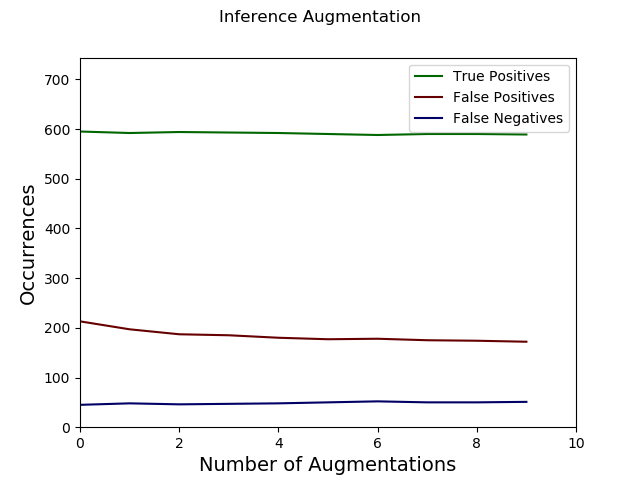
\includegraphics[width=0.45\linewidth]{./figures/Kasthuri-test-augmentation.png}
	\caption{The number of false positives decreases with our data augmentation scheme. The benefit of augmentation gradually decreases with the number of random examples.}
	\label{fig:test-augmentation}
\end{figure}
